\documentclass[10pt]{beamer}
\usetheme[
%%% options passed to the outer theme
%    progressstyle=movCircCnt,   %either fixedCircCnt, movCircCnt, or corner
%    rotationcw,          % change the rotation direction from counter-clockwise to clockwise
%    shownavsym          % show the navigation symbols
  ]{AAUsimple}
  
% If you want to change the colors of the various elements in the theme, edit and uncomment the following lines
% Change the bar and sidebar colors:
%\setbeamercolor{AAUsimple}{fg=red!20,bg=red}
%\setbeamercolor{sidebar}{bg=red!20}
% Change the color of the structural elements:
%\setbeamercolor{structure}{fg=red}
% Change the frame title text color:
%\setbeamercolor{frametitle}{fg=blue}
% Change the normal text color background:
%\setbeamercolor{normal text}{fg=black,bg=gray!10}
% ... and you can of course change a lot more - see the beamer user manual.
\usepackage{atbegshi}
\usepackage{anyfontsize}

\usepackage[utf8]{inputenc}
\usepackage[english]{babel}
\usepackage[T1]{fontenc}
% Or whatever. Note that the encoding and the font should match. If T1
% does not look nice, try deleting the line with the fontenc.
\usepackage{helvet}
\usepackage{tikz}

% Defines new environments such as equation,
% align and split 
\usepackage{amsmath}
\usepackage{relsize}
% Adds new math symbols
\usepackage{amssymb}

% colored hyperlinks
\newcommand{\chref}[2]{%
  \href{#1}{{\usebeamercolor[bg]{AAUsimple}#2}}%
}

\title{\large{Attitude and Position Control of a Quadcopter in a Networked Distributed System}}

\subtitle{%\\  \vspace{0.1cm} 
    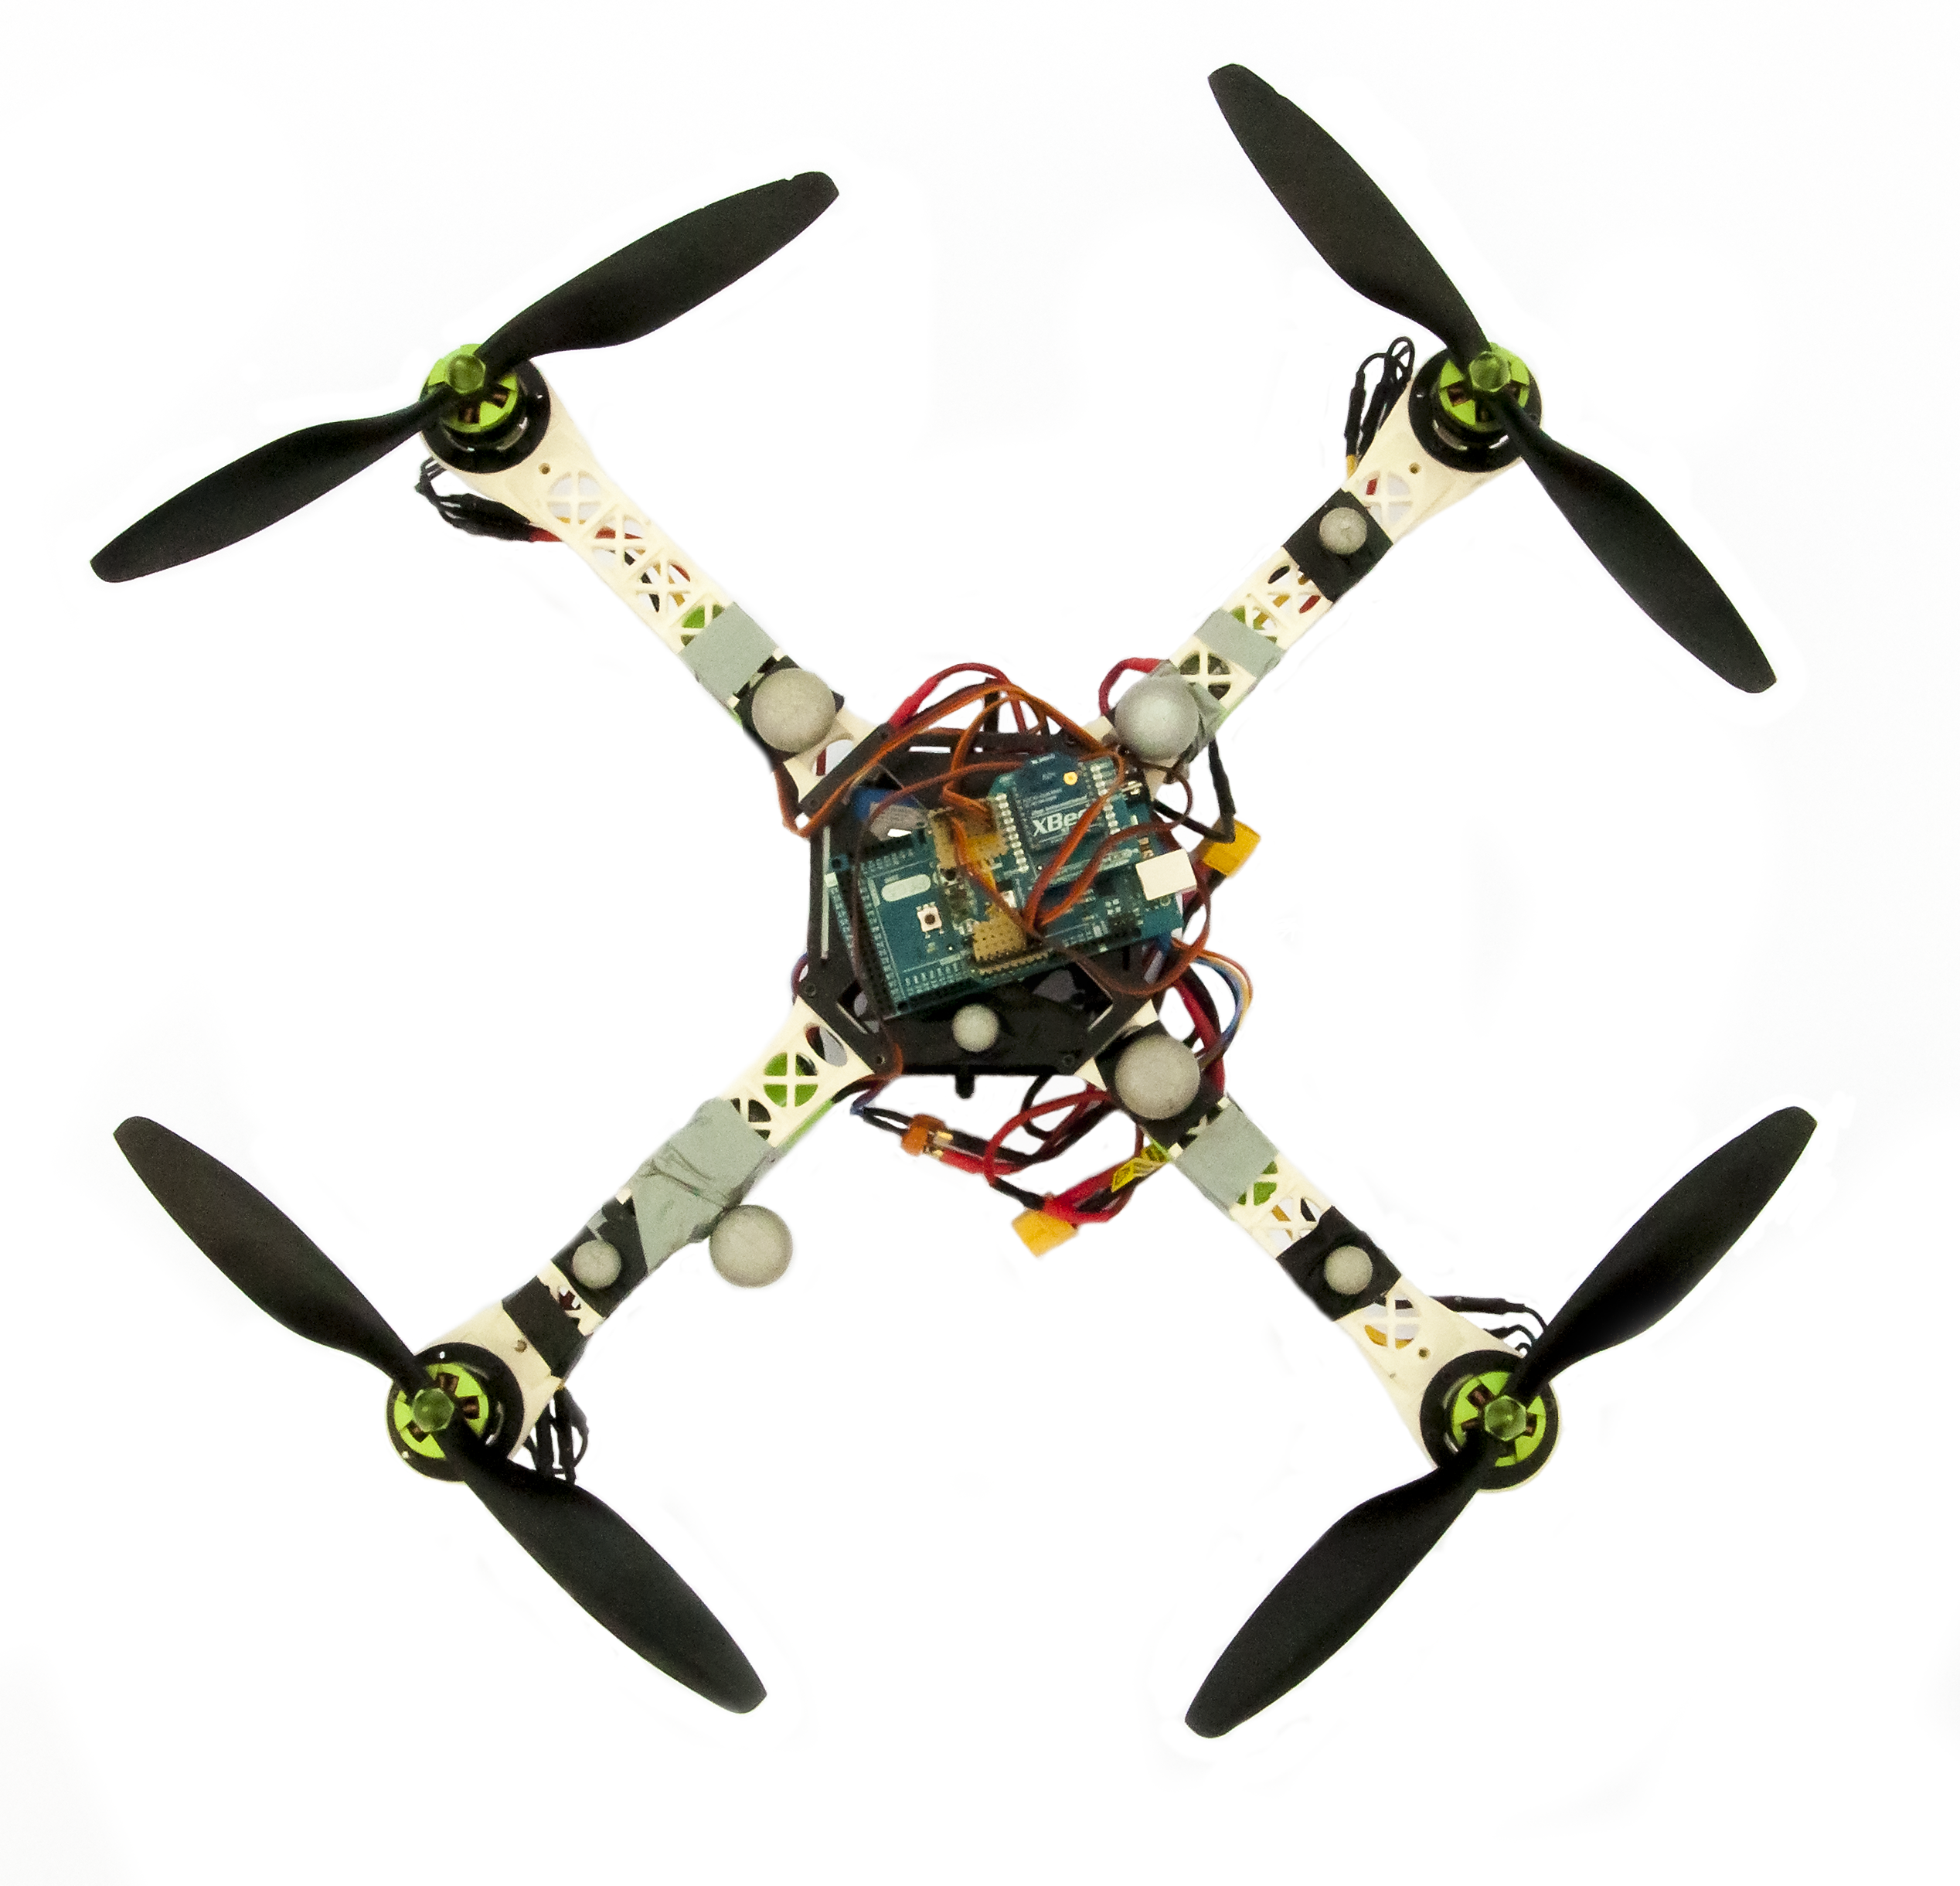
\includegraphics[width=6cm]{figures/quadcopter}}  % could also be a conference name

%\date{\today}
%
\author{
    \footnotesize{Alejandro Alonso García, Amalie Vistoft Petersen, Andrea Victoria Tram Løvemærke, Niels Skov Vestergaard, Noelia Villarmarzo Arruñada}}
%
%% - Give the names in the same order as they appear in the paper.
%% - Use the \inst{?} command only if the authors have different
%%   affiliation. See the beamer manual for an example
%
%\institute[
%%  {\includegraphics[scale=0.2]{aau_segl}}\\ %insert a company, department or university logo
%  Dept.\ of Electronic Systems\\
%  Aalborg University\\
%  Denmark
%] % optional - is placed in the bottom of the sidebar on every slide
%{% is placed on the bottom of the title page
%  Department of Electronic Systems\\
%  Aalborg University\\
%  Denmark
%  
%  %there must be an empty line above this line - otherwise some unwanted space is added between the university and the country (I do not know why;( )
%}

% specify a logo on the titlepage (you can specify additional logos an include them in 
% institute command below
%\pgfdeclareimage[height=1.5cm]{titlepagelogo}{AAUgraphics/aau_logo_new} % placed on the title page
%%\pgfdeclareimage[height=1.5cm]{titlepagelogo2}{AAUgraphics/aau_logo_new} % placed on the title page
%\titlegraphic{% is placed on the bottom of the title page
%  \pgfuseimage{titlepagelogo}
%%  \hspace{1cm}\pgfuseimage{titlepagelogo2}
%}

\begin{document}
%%%%%%%%%%%%%%%%%%%%%%%%%%%%%%%%%%%%%%%%%%%%%%%%%%%%%
%             UNITS, EQUATIONS AND TEXT             %
%%%%%%%%%%%%%%%%%%%%%%%%%%%%%%%%%%%%%%%%%%%%%%%%%%%%%

%%Macro for 'where'enviroment has been improved by Andrea :-)

%Units:
\newcommand{\unit}[1]{&& \left[\si{#1}\right]} %\newcommand{\unit}[1]{[\si{#1}]}             <<| Use these if you want equations to be
\newcommand{\unitWh}[1]{[\si{#1}]}             %\newcommand{\eq}[2]{&&\si{#1} &= \si{#2}&&}  <<| centered.. .. will appear scrambled
\newcommand{\numUnit}[1]{\ \si{#1}&}           %                                               | from one equation to the next though..
%Equation:                                     %                                               | and does not work with long equations.. :/
\newcommand{\eq}[2]{\si{#1} &= \si{#2}}
\newcommand{\arw}{&& &\Updownarrow&&}
\newcommand{\eqOne}[2]{\si{#1} &= \si{#2} &\nonumber\\}
\newcommand{\eqTwo}[1]{&\ \ \ \ \si{#1}&}
\newcommand{\eqThree}[1]{&\ \ \ \ \si{#1}&}
%Text:
\newcommand{\tx}[1]{\text{#1}}
%Vectors
\renewcommand{\vec}[1]{\boldsymbol{\mathbf{#1}}}
%Vertical line in equations ie. |_x=y (whereTwo stacks two equalities at the line)



\newcommand{\oleStreg}[1]{ \left.\right\vert\rule{0cm}{.4cm}_{\substack{\rule{0cm}{.15cm}\\ #1 }} }

\newcommand{\oleStregTwo}[2]{ \left.\rule{0cm}{.7cm}\right\vert\rule{0cm}{.7cm}_{\substack{#1 \rule{0cm}{.2cm}\\\vspace{-.1cm}\\ #2}} }
%
%\newenvironment{where}{\indent Where:\\}{}
%\newcommand{\va}[3]{\hspace{16mm} \begin{tabular}{p{40pt} p{360pt} l} {#1} & {#2} & \ifthenelse{\isempty{#3}}{}{[{#3}]} \\
%	\end{tabular}\\}





%%%%%%%%%%%%%%%%%%%%%%%%%%%%%%%%%%%%%%%%%%%%%%%%%%%%%
%              SETTING UP NOTE BOXES                %
%%%%%%%%%%%%%%%%%%%%%%%%%%%%%%%%%%%%%%%%%%%%%%%%%%%%%
%\specialcomment{note}{\[}{\]}
%%{\begin{tcolorbox}
%%                      [grow to right by  = 1.5 cm
%%                      ]}{\vspace{-.3 cm}\end{tcolorbox}}
%
%\newcommand{\toggleNotes}[1]
%{
%  \ifthenelse{\equal{#1}{off}}{\excludecomment{note}}{}
%}

%%%%%%%%%%%%%%%%%%%%%%%%%%%%%%%%%%%%%%%%%%%%%%%%%%%%%
%                 TIKZ SETTINGS                     %
%%%%%%%%%%%%%%%%%%%%%%%%%%%%%%%%%%%%%%%%%%%%%%%%%%%%%
%\usetikzlibrary{arrows.meta}
\tikzset{
  block/.style    = {draw, thick, rectangle,
                     minimum height = 2.1em,
                     minimum width = 1.7em},
  sum/.style      = {draw, circle, inner sep=1.5pt},
}

%%%%%%%%%%%%%%%%%%%%%%%%%%%%%%%%%%%%%%%%%%%%%%%%%%%%%
%                  REFERENCES                       %
%%%%%%%%%%%%%%%%%%%%%%%%%%%%%%%%%%%%%%%%%%%%%%%%%%%%%

%Chapter
\newcommand{\Chapref}[1]{\emph{Chapter \ref{#1}}}
\newcommand{\chapref}[1]{\emph{chapter \ref{#1}}}
%Section
\newcommand{\Secref}[1]{\emph{Section \ref{#1}}}
\newcommand{\secref}[1]{\emph{section \ref{#1}}}
%subSection
\newcommand{\Subsecref}[1]{\emph{Subsection \ref{#1}}}
\newcommand{\subsecref}[1]{\emph{subsection \ref{#1}}}
%Appendix
\newcommand{\Appref}[1]{\emph{Appendix \ref{#1}}}
\newcommand{\appref}[1]{\emph{appendix \ref{#1}}}
%Listings
\newcommand{\Coderef}[1]{\emph{Listings: \ref{#1}}}
\newcommand{\coderef}[1]{\emph{listings: \ref{#1}}}
%Figure:
\newcommand{\Figref}[1]{\emph{Figure \ref{#1}}}
\newcommand{\figref}[1]{\emph{figure \ref{#1}}}
%Table:
\newcommand{\Tableref}[1]{\emph{Table \ref{#1}}}
\newcommand{\tableref}[1]{\emph{table \ref{#1}}}

%Expressions:
\newcommand{\Expr}[1]{\emph{Expression (\ref{#1})}}
\newcommand{\expr}[1]{\emph{expression (\ref{#1})}}

%Equations:
%1 equation:
\newcommand{\Eqref}[1]{\emph{Equation (\ref{#1})}}
\renewcommand{\eqref}[1]{\emph{equation (\ref{#1})}}
%2 equations:
\newcommand{\EqrefTwo}[2]{\emph{Equation (\ref{#1})} and \emph{(\ref{#2})}}
\newcommand{\eqrefTwo}[2]{\emph{equation (\ref{#1})} and \emph{(\ref{#2})}}
%3 equations:
\newcommand{\EqrefThree}[3]{\emph{Equation (\ref{#1})}, \emph{(\ref{#2})} and \emph{(\ref{#3})}}
\newcommand{\eqrefThree}[3]{\emph{equation (\ref{#1})}, \emph{(\ref{#2})} and \emph{(\ref{#3})}}
%4 equations:
\newcommand{\EqrefFour}[4]{\emph{Equation (\ref{#1})}, \emph{(\ref{#2})}, \emph{(\ref{#3})} and \emph{(\ref{#4})}}
\newcommand{\eqrefFour}[4]{\emph{equation (\ref{#1})}, \emph{(\ref{#2})}, \emph{(\ref{#3})} and \emph{(\ref{#4})}}
%5 equations:
\newcommand{\EqrefFive}[5]{\emph{Equation (\ref{#1})}, \emph{(\ref{#2})}, \emph{(\ref{#3})}, \emph{(\ref{#4})} and \emph{(\ref{#5})}}
\newcommand{\eqrefFive}[5]{\emph{equation (\ref{#1})}, \emph{(\ref{#2})}, \emph{(\ref{#3})}, \emph{(\ref{#4})} and \emph{(\ref{#5})}}
%6 equations:
\newcommand{\EqrefSix}[6]{\emph{Equation (\ref{#1})}, \emph{(\ref{#2})}, \emph{(\ref{#3})}, \emph{(\ref{#4})}, \emph{(\ref{#5})} and \emph{(\ref{#6})}}
\newcommand{\eqrefSix}[6]{\emph{equation (\ref{#1})}, \emph{(\ref{#2})}, \emph{(\ref{#3})}, \emph{(\ref{#4})}, \emph{(\ref{#5})} and \emph{(\ref{#6})}}
%7 equations:
\newcommand{\EqrefSeven}[7]{\emph{Equation (\ref{#1})}, \emph{(\ref{#2})}, \emph{(\ref{#3})}, \emph{(\ref{#4})}, \emph{(\ref{#5})}, \emph{(\ref{#6})} and \emph{(\ref{#7})}}
\newcommand{\eqrefSeven}[7]{\emph{equation (\ref{#1})}, \emph{(\ref{#2})}, \emph{(\ref{#3})}, \emph{(\ref{#4})}, \emph{(\ref{#5})}, \emph{(\ref{#6})} and \emph{(\ref{#7})}}


\newcommand{\newpar}{\par \vspace{0.4cm}}


\usepackage{xifthen}

\newenvironment{where}{\indent Where:\\}{}
\newcommand{\va}[3]
{
  \hspace{-18mm}
  \begin{tabular}{p{35pt} p{345pt} l}
    { $#1$ } & { #2 } & \ifthenelse{\isempty{ #3 }}  {}  {\si{[#3]}}
  \end{tabular}
}



% the titlepage
%{\aauwavesbg%
\begin{frame}[plain,noframenumbering] % the plain option removes the header from the title page
  \titlepage
\end{frame}%}

% TOC
\begin{frame}{Agenda}{}
\tableofcontents
\end{frame}

%%%%%%%%%%%%%%%%
\section{Introduction}

\subsection{}
\begin{frame}{Introduction}{}
\begin{figure}[H]
    \centering
    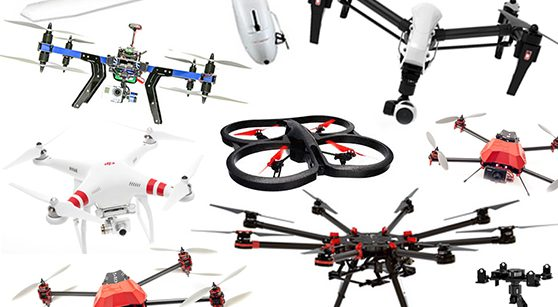
\includegraphics[width=.6\linewidth]{figures/multicopters}
\end{figure}
\uncover<2>{
    \begin{itemize}
        \item 
    \end{itemize}
}
\end{frame}

\begin{frame}{Introduction}{Prototype}
    \begin{figure}[H]
        \centering
        \includegraphics[width=.45\linewidth]{figures/SDPhotowithNumbers}
    \end{figure}
\uncover<2>{  
     \begin{itemize}
         \item  
         \item
       \end{itemize}
}     
\end{frame}

%%%%%%%%%%%%%%%%
\section{Model}
\subsection{Attitude Model}
\begin{frame}{Model}{Attitude Model}
    \only<1>{
        \begin{figure}[H]
            \includegraphics[width=0.6\textwidth]{figures/dronediagram1}
        \end{figure}            
    }
    \only<2>{
        \begin{figure}[H]
            \includegraphics[width=0.6\textwidth]{figures/dronediagram2}
        \end{figure}            
    }
    \only<3>{
        \begin{figure}[H]
            \includegraphics[width=0.6\textwidth]{figures/dronediagram3}
        \end{figure}            
    }
    \only<4>{
        \begin{figure}[H]
            \includegraphics[width=0.6\textwidth]{figures/dronediagram4}
        \end{figure}            
    }
    \only<5>{
        \begin{figure}[H]
            \includegraphics[width=0.6\textwidth]{figures/dronediagram5}
        \end{figure}            
    }
    \only<6>{
        \begin{figure}[H]
            \includegraphics[width=0.6\textwidth]{figures/dronediagram6}
        \end{figure}            
    }
    \only<7>{
        \begin{figure}[H]
            \includegraphics[width=0.6\textwidth]{figures/dronediagram7}
        \end{figure}            
    }
    \only<8>{
        \begin{figure}[H]
            \includegraphics[width=0.6\textwidth]{figures/dronediagram8}
        \end{figure}            
    }   
\end{frame}

\begin{frame}{Model}{Attitude Model}
     \begin{itemize}
         \item Dynamic Equations
        \end{itemize}
    \uncover<2-4>{            
    \begin{flalign}
    J \alpha=\sum\tau \nonumber
    \end{flalign}
    }
    \uncover<3-4>{
        \begin{align}
        J_x \ddot{\phi}&=(F_4-F_2) L \nonumber \\
        J_y \ddot{\theta}&=(F_1-F_3) L \nonumber \\
        J_z \ddot{\psi}&=\tau_1-\tau_2+\tau_3-\tau_4 \nonumber
        \end{align}
    }
        \uncover<4>{
        \begin{align}
        J_x \ddot{\phi}&=k_\mathrm{th} (\omega^2_4-\omega^2_2)  L \nonumber\\
        J_y \ddot{\theta}&=k_\mathrm{th} (\omega^2_1-\omega^2_3)  L \nonumber\\
        J_z \ddot{\psi}&=k_\mathrm{d} (\omega^2_1-\omega^2_2+\omega^2_3-\omega^2_4) \nonumber
        \end{align}
        }    
    
\end{frame}

%%
% TOC
\begin{frame}{Agenda}{}
    \tableofcontents
\end{frame}

%%
\subsection{Translational Model}
\begin{frame}{Model}{Free Body Diagram}	

    \only<1>{
        \begin{figure}[H]
            \includegraphics[width=1\textwidth]{figures/dronediagram1}
        \end{figure}            
    }
    \only<2>{
        \begin{figure}[H]
            \includegraphics[width=1\textwidth]{figures/dronediagram2}
        \end{figure}            
    }
    \only<3>{
        \begin{figure}[H]
            \includegraphics[width=1\textwidth]{figures/dronediagram3}
        \end{figure}            
    }
    \only<4>{
        \begin{figure}[H]
            \includegraphics[width=1\textwidth]{figures/dronediagram4}
        \end{figure}            
    }
    \only<5>{
        \begin{figure}[H]
            \includegraphics[width=1\textwidth]{figures/dronediagram5}
        \end{figure}            
    }
    \only<6>{
        \begin{figure}[H]
            \includegraphics[width=1\textwidth]{figures/dronediagram6}
        \end{figure}            
    }
    \only<7>{
        \begin{figure}[H]
            \includegraphics[width=1\textwidth]{figures/dronediagram7}
        \end{figure}            
    }
    \only<8>{
        \begin{figure}[H]
            \includegraphics[width=1\textwidth]{figures/dronediagram8}
        \end{figure}            
    }
    \only<9>{
        \begin{figure}[H]
            \includegraphics[width=1\textwidth]{figures/dronediagram9}
        \end{figure}            
    }
\end{frame}

\begin{frame}{Translational Model}{}
    Something with rotation
\end{frame}

\begin{frame}{Translational Model}{}
    equations
\end{frame}

\subsection{Linearization of the Model}
\begin{frame}{Linearization of the Model}{}
    
\end{frame}

%%%%%%%%%%%%%%%%
\section{Network}
\begin{frame}{Network}{}
    talk about protocol 
\end{frame}

\begin{frame}{Network}{Main Issues}
    \begin{itemize}
        \item Delay
    \end{itemize}
    \begin{itemize}
        \item Missed packets
    \end{itemize}
    
    \begin{minipage}{\linewidth}
        \begin{minipage}{0.49\linewidth}
            \begin{figure}[H]
                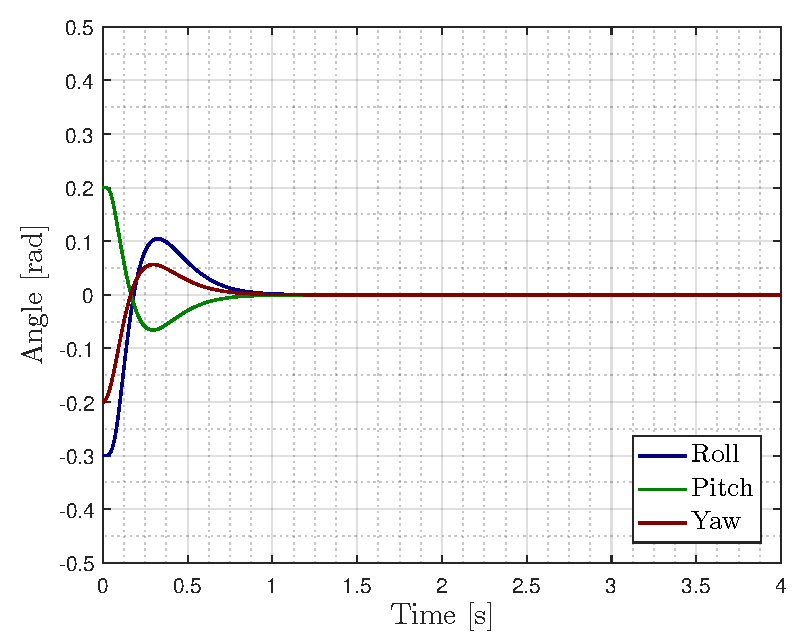
\includegraphics[width=1\textwidth]{figures/nonetwork}
            \end{figure}
            \centering
            Control design only taking the model into account
        \end{minipage}
        \hspace{0.03\linewidth}
        \begin{minipage}{0.49\linewidth}
            \begin{figure}[H]
                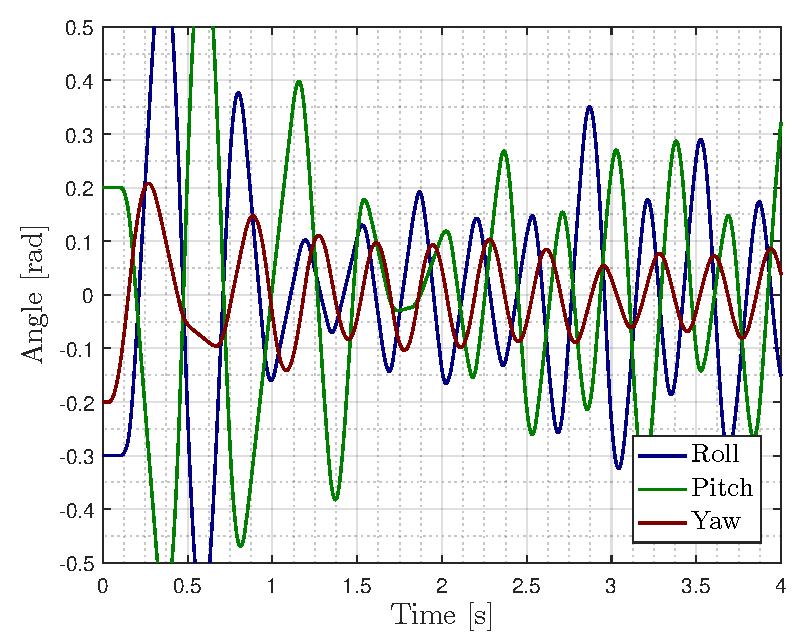
\includegraphics[width=1\textwidth]{figures/network}
            \end{figure}  
            \centering
            Same controller with the effect of the network                   
        \end{minipage}
    \end{minipage}  
\end{frame}

%%
% TOC
\begin{frame}{Agenda}{}
    \tableofcontents
\end{frame}

%%
%%%%%%%%%%%%%%%%
\section{Control Solution}
\begin{frame}{Control Solution}{}

\end{frame}

\subsection{Attitude Controller}
\begin{frame}{Control Solution}{Attitude Controller}
    
\end{frame}

%%
% TOC
\begin{frame}{Agenda}{}
    \tableofcontents
\end{frame}

%%
\subsection{Translational Controller}
\begin{frame}{Control Solution}{Translational Controller}
    \begin{figure}[H]
        
\includegraphics[width=1\textwidth]{figures/TranslationalControlDiagramSmall}
    \end{figure}      
\end{frame}

\begin{frame}{Control Solution}{Translational Controller}
    transfer functions with block diagram
\end{frame}

\begin{frame}{Control Solution}{Translational Controller}
    put three root locus      
\end{frame}

\begin{frame}{Control Solution}{Translational Controller}
    consideration of bandwidth
    equations for velocity controllers
    equations for position controllers
\end{frame}


%%%%%%%%%%%%%%%%
\section{Implementation}
\begin{frame}{Implementation}{}
    FreeRTOS, tasks
\end{frame}

\begin{frame}{Implementation}{Schedule}
    old 35ms 
\end{frame}

\begin{frame}{Implementation}{Schedule}
   new, 25ms, less sampling freq. 
\end{frame}

\begin{frame}{Implementation}{Schedule}
   comparison oscilloscope
\end{frame}
    
    
%%
% TOC
\begin{frame}{Agenda}{}
    \tableofcontents
\end{frame}

%%
%%%%%%%%%%%%%%%%
\section{Results}
\begin{frame}{Results}{Attitude Controller Simulations}
    \begin{figure}[H]
        %
\includegraphics[width=1\textwidth]{figures/TranslationalControlDiagramSmall}
    \end{figure}    
    \begin{figure}[H]
        %
\includegraphics[width=1\textwidth]{figures/TranslationalControlDiagramSmall}
    \end{figure}    
\end{frame}

\begin{frame}{Results}{Translational Controllers Simulations}
    \begin{figure}[H]
        %
\includegraphics[width=1\textwidth]{figures/TranslationalControlDiagramSmall}
    \end{figure}    
\end{frame}

\begin{frame}{Results}{Attitude Controller Functional Tests}
    \begin{figure}[H]
        %
\includegraphics[width=1\textwidth]{figures/TranslationalControlDiagramSmall}
    \end{figure}    
    \begin{figure}[H]
        %
\includegraphics[width=1\textwidth]{figures/TranslationalControlDiagramSmall}
    \end{figure}    
\end{frame}

%%%%%%%%%%%%%%%%
\section{Conclusion}
\begin{frame}{Conclusion}{}
    \begin{itemize} 
        \item[-] Similar to SEMCON
        \item[-]
        \item[-]
    \end{itemize}   
\end{frame}

%{\aauwavesbg
\begin{frame}[plain,noframenumbering]
    \finalpage{\large{Attitude and Position Control of a Quadcopter in a Networked Distributed System}}
\end{frame}%}
%%%%%%%%%%%%%%%%

\end{document}
